\documentclass[reprint,english,notitlepage]{revtex4-1}  % defines the basic parameters of the document

% if you want a single-column, remove reprint

% allows special characters (including æøå)
\usepackage[utf8]{inputenc}
\usepackage[english]{babel}
\usepackage{float}
\usepackage{algorithm}
\usepackage[noend]{algpseudocode}
%% note that you may need to download some of these packages manually, it depends on your setup.
%% I recommend downloading TeXMaker, because it includes a large library of the most common packages.

\usepackage{physics,amssymb}  % mathematical symbols (physics imports amsmath)
\usepackage{graphicx}         % include graphics such as plots
\usepackage{xcolor}           % set colors
\usepackage{hyperref}         % automagic cross-referencing (this is GODLIKE)
\usepackage{tikz}             % draw figures manually
\usepackage{listings}         % display code
\usepackage{subfigure}        % imports a lot of cool and useful figure commands

% defines the color of hyperref objects
% Blending two colors:  blue!80!black  =  80% blue and 20% black
\hypersetup{ % this is just my personal choice, feel free to change things
    colorlinks,
    linkcolor={red!50!black},
    citecolor={blue!50!black},
    urlcolor={blue!80!black}}

%% Defines the style of the programming listing
%% This is actually my personal template, go ahead and change stuff if you want
\lstset{ %
	inputpath=,
	backgroundcolor=\color{white!88!black},
	basicstyle={\ttfamily\scriptsize},
	commentstyle=\color{magenta},
	language=Python,
	morekeywords={True,False},
	tabsize=4,
	stringstyle=\color{green!55!black},
	frame=single,
	keywordstyle=\color{blue},
	showstringspaces=false,
	columns=fullflexible,
	keepspaces=true}


%% USEFUL LINKS:
%%
%%   UiO LaTeX guides:        https://www.mn.uio.no/ifi/tjenester/it/hjelp/latex/ 
%%   mathematics:             https://en.wikibooks.org/wiki/LaTeX/Mathematics

%%   PHYSICS !                https://mirror.hmc.edu/ctan/macros/latex/contrib/physics/physics.pdf

%%   the basics of Tikz:       https://en.wikibooks.org/wiki/LaTeX/PGF/TikZ
%%   all the colors!:          https://en.wikibooks.org/wiki/LaTeX/Colors
%%   how to draw tables:       https://en.wikibooks.org/wiki/LaTeX/Tables
%%   code listing styles:      https://en.wikibooks.org/wiki/LaTeX/Source_Code_Listings
%%   \includegraphics          https://en.wikibooks.org/wiki/LaTeX/Importing_Graphics
%%   learn more about figures  https://en.wikibooks.org/wiki/LaTeX/Floats,_Figures_and_Captions
%%   automagic bibliography:   https://en.wikibooks.org/wiki/LaTeX/Bibliography_Management  (this one is kinda difficult the first time)
%%   REVTeX Guide:             http://www.physics.csbsju.edu/370/papers/Journal_Style_Manuals/auguide4-1.pdf
%%
%%   (this document is of class "revtex4-1", the REVTeX Guide explains how the class works)


%% CREATING THE .pdf FILE USING LINUX IN THE TERMINAL
%% 
%% [terminal]$ pdflatex template.tex
%%
%% Run the command twice, always.
%% If you want to use \footnote, you need to run these commands (IN THIS SPECIFIC ORDER)
%% 
%% [terminal]$ pdflatex template.tex
%% [terminal]$ bibtex template
%% [terminal]$ pdflatex template.tex
%% [terminal]$ pdflatex template.tex
%%
%% Don't ask me why, I don't know.

\begin{document}
\title{This is a Very Important Title!}   % self-explanatory
\author{Person McSomething}               % self-explanatory
\date{\today}                             % self-explanatory
\noaffiliation                            % ignore this
\begin{abstract}                          % marks the beginning of the abstract
This abstract is abstract.                % the body of the abstract
\end{abstract}                            % marks the end of the abstract
\maketitle                                % creates the title, author, date & abstract

If you want to learn more about using \LaTeX, you should check UiO's official tutorials:
\url{https://www.mn.uio.no/ifi/tjenester/it/hjelp/latex/}

If you are familiar with \LaTeX\ and you want to learn more about the REVTeX4-1 document class, check:
\url{http://www.physics.csbsju.edu/370/papers/Journal_Style_Manuals/auguide4-1.pdf}


% the fundamental components of scientific reports:
\section{Introdukson}

\section{Teori}   % (optional)
Legger vi til flere partikler i systemet som kan påvirke hverandre med Coloumb krefter, så får vi en bevegelse som ser slik ut:
$$
\ddot{x}_i -\omega_{0,i} \ddot{y}_i-\frac{1}{2}\omega_{z,i}^2x_i-k_e\frac{q_e}{m_i}\sum_{j\neq i}q_j\frac{x_i-x_j}{|\vec{r}_i-\vec{r}_j|^3}=0
$$
$$
\ddot{y}_i -\omega_{0,i} \ddot{x}_i-\frac{1}{2}\omega_{z,i}^2y_i-k_e\frac{q_e}{m_i}\sum_{j\neq i}q_j\frac{y_i-y_j}{|\vec{r}_i-\vec{r}_j|^3}=0
$$
$$
\ddot{z}_i+w_{z,i}^20z_i-k_e\frac{q_e}{m_i}\sum_{j\neq i}q_j\frac{z_i-z_j}{|\vec{r}_i-\vec{r}_j|^3}=0
$$
Som det vil bli forklart dypere hvordan i Metode-delen skal vi bruke to numeriske metoder for å simulere banen. Den ene er Eulers meotde og den andre er Runge Kutta 4. For Euler-Cromer vil vi ha en feilorden av orden $O(h^)$
\section{Metode}
\subsection*{Enpartikkelsystemet}
Vi starter først med et enpartikkelsystem. Vi setter partikkelen i samme posisjon som i den analytiske delen, altså
$$
\vec{r}(0)=\begin{bmatrix}
x_0 \\ 0 \\0
\end{bmatrix}
$$
og
$$
\vec{v}=\begin{bmatrix}
0\\v_0\\0
\end{bmatrix}
$$
hvor vi setter $x_0=1\mu m$ og $v_0=1\frac{\mu m}{\mu s}$ for enkelhetsskyld. Vi bruker så at det elektriske feltet kan skrives som
$$
\vec{E}=\begin{Bmatrix}
V0\frac{x}{d^2} \\V_0 \frac{y}{d^2}\\-2V_0 \frac{z}{d^2}
\end{Bmatrix}
$$

og det magnetiske feltet er $\vec{B}=(0,0,B_0)$. Vi vet også at den eksterne kraften er gitt som
$$
\vec{F}_{eks}=q\vec{E}+q\vec{v}\cross \vec{B}
$$
og slik kan vi regne ut den eksterne kraften.
Så skal vi bruke dette som kraften når vi bruker de numeriske metodene.
Vi starter med Eulers metode som er ganske rett fram:
\begin{algorithm}[H]
	\begin{algorithmic}
		\State Some maths, e.g $f(x) = x^2$. 
		\For{$i = 0, 1, ..., N-1$}
		\State $$
		r_{i+1}\leftarrow r_i+v_i \cdot h
		$$
		\State $$
		v_{i+1}\leftarrow v_i+\frac{F(r_i, v_i)}{m}\cdot h
		$$
		\EndFor
	\end{algorithmic}
\end{algorithm}
Runge Kutta 4 er litt mer komplisert:
\begin{algorithm}[H]
	\begin{algorithmic}
		\State Some maths, e.g $f(x) = x^2$. 
		\For{$i = 0, 1, ..., N-1$}
		\State $$
		R\leftarrow r_i
		$$$$
		V\leftarrow v_i
		$$$$
		vk_1\leftarrow h\cdot F(r_i, v_i)
		$$$$
		rk_1\leftarrow h\cdot v_i
		$$$$
		v_{i+1}\leftarrow V+vk1/2.0
		$$$$
		r_{i+1}\leftarrow R+rk1/2.0
		$$
		$$
		vk_2\leftarrow h\cdot \frac{F(r_{i+1},v_{i+1})}{m}
		$$$$
		rk_2\leftarrow h\cdot v_{i+1}
		$$
		$$
		v_{i+1}\leftarrow V+vk_2/2
		$$$$
		r_{i+1}=R+rk_2/2
		$$
		$$
		vk_3\leftarrow h\cdot F(r_{i+1}, v_{i+1})/m
		$$$$
		rk_3\leftarrow h\cdot v_{i+1}
		$$
		$$
		v_{i+1}\leftarrow V+vk_3$$$$
		r_{i+1}\leftarrow R+rk_3
		$$
		$$
		vk_4\leftarrow h\cdot  F(r_{i+1}, v_{i+1})/m$$$$
		rk_4=h\cdot v_{i+1}
		$$
		$$
		v_{i+1}=V+(vk_1+2vk_2+2vk_3+vk_4)/6$$$$
		r_{i+1}=R+(rk_1+2rk_2+2rk_3+rk_4)/6;
		$$
		\EndFor
	\end{algorithmic}
\end{algorithm}
\subsection*{Topartikkelsystemet}
I disse simulasjonene vil vi kun bruke Runge Kutta 4.
\section{Resultater}

\subsection*{Énpartikkelsystemet}
Vi fikk at i ènpartikkelsystemet så ble posisjonene som gitt i figur \ref{r1pos}.
\begin{figure}
	\label{r1pos}
	\centering 
	\includegraphics[scale=0.4]{../pythonplots/r1pos.pdf}
	\caption{Posisjonene fordelt i x,y og z-retning for en partikkel alene i systemet.}
\end{figure}
Av den analytiske løsningen var $\omega_z=\frac{2qV_0}{md^2}$ som med våre verdier gir $\omega_z=0,982Hz$.
Hastigheten fra den numeriske løsningen ble som i figur \ref{v1z}.
\begin{figure}
	\label{v1z}
	\centering 
	\includegraphics[scale=0.4]{../pythonplots/vz.pdf}
	\caption{Hastigheten i z-retning for en partikkel alene i fella.}
\end{figure}
De relative feilene for Eulers metode over tiden ble seende ut som i figur \ref{errEu}, mens de relative feilene for Runge-Kutta 4 er gitt i figur \ref{errRK4}
\begin{figure}[H]
	\label{errEu}
	\centering 
	\includegraphics[scale=0.4]{../pythonplots/RelerrEu.pdf}
	\caption{De relative feilene over tiden for ulike tidssteg ved bruke av Eulers metode}
\end{figure}
\begin{figure}[H]
	\label{errRK4}
	\centering 
	\includegraphics[scale=0.4]{../pythonplots/RelerrRK4.pdf}
	\caption{De relative feilene over tiden for ulike tidssteg ved å bruke Runge Kutta 4}
\end{figure}

\subsection*{To-partikkelsystemet}
Partiklene uten interaksjon vil se ut som i figur \ref{r2noint} i xy-planet.
\begin{figure}
	\label{r2noint}
	\centering 
	\includegraphics[scale=0.4]{../pythonplots/xypartnoint.pdf}
	\caption{To partikler som ikke gir forveksler kraft med hverandre i feltet}
\end{figure}
Partiklene med interaksjon ble derimot seende ut som på figur \ref{r2int} i xy-planet
\begin{figure}
	\label{r2int}
	\centering 
	\includegraphics[scale=0.4]{../pythonplots/xypartint.pdf}
	\caption{To partikler i feltet som også kan virke på hverandre.}
\end{figure}
I tre dimensjoner vil banene se ut som i figur \ref{3dnoint} uten partikkelinteraksjon, mens banene med partikkelinteraksjon vil se ut som de i figur \ref{3dint}.
\begin{figure}
	\label{3dnoint}
	\centering
	\includegraphics[scale=0.4]{../pythonplots/3dr2noint.pdf}
	\caption{Partiklenes baner i 3 dimensjoner uten partikkelinteraksjon.}
\end{figure}
\begin{figure}
	\label{3dint}
	\centering
	\includegraphics[scale=0.4]{../pythonplots/3dr2int.pdf}
	\caption{Partikelenes baner i 3 dimensjoner med partikkelinteraksjon.}
\end{figure}
\section{Diskusjon}
\subsection*{Énpartikkelsystemet}
Vi ser at når for små tidsteg som $h=10^{-3}$ og $h=10^{-4}$, så fungerer både Eulers metode og Runge Kutta 4 ganske bra. Når vi derimot beveger oss fra $h=10^{-2}$ og oppover blir Euler mer og mer unøyaktig og feilen stiger lineært med tiden. Dette er fordi Euler ikke er god på å rette seg i oscillerende systemer.
\newline Runge-Kutta 4 derimot er holder seg ganske nærme null for alle testene av tidsteg utenom $h=1$, som gir mening siden $h$ burde være mindre enn 1 for at det skal konvergere.
\subsection*{Topartikkelsystemet}
Vi ser at når partikkelene ikke påvirker hverandre følger de baner som likner enpartikkelsystemet, som kan tyde på at denne simuleringen fungerer. Man kan tross alt se på de to partiklene som to uavhengige énpartikkelsystemer. Når vi skrur på interaksjonen derimot, så ser vi noe ganske annet. Vi kan fortsatt se noen tendenser til et liknende mønster, for eksempel at det fortsatt er sirkelbevegelse inni en større sirkelbevegelse, men vi ser også at partiklene har mye større baner enn før. Dette kan være fordi partiklene startet kun noen mikrometer nærme hverandre og partikkelkraften mellom dem har derfor blitt veldig sterk og skutt dem ut i større baner. Her har de kanskje blitt langt fra hverandre og kreftene mellom dem har blitt mindre. Da vil de eksterne kreftene ha mer å si igjen og de begynner å likne mer på énpartikkelsystemer igjen. Da vil de også gå i baner igjen, men større baner enn før, som stemmer med figuren siden vi gikk fra en bane med radius på rundt $1\mu m$ til en bane med radius rundt $10\mu m$.
\section{Conklusjon}
% acknowledgements (optional)
\begin{acknowledgments}  % if you disagree with the spelling, blame Americans
I would like thank myself for writing this beautiful document.
\end{acknowledgments}


%% When it comes to the bibliography I personally generate it using BibLaTeX. (see the link above if you're interested)
%% You're obviously allowed to create the references section however you like.
%% I'll keep it simple here.
\section*{References}  % the asterisk (*) after \section makes the section numbering go away
\begin{itemize}
\item[-]Reference 1
\item[-]Reference 2
\end{itemize}

\newpage
%% if you want to include an appendix, this is how you do it
\appendix
\section{Name of appendix}
This will be the body of the appendix.
\section{This is another appendix}\label{appendix}
Tada.
%% all \section commands following \appendix are automatically taken as appendices

%% Note that \label{appendix} command on line 115. What this does is setup a reference point for LaTeX that you can
%% access wherever you want using \ref{appendix}.
%% You can place labels on most environments such as equations, figures, tables, etc.

\clearpage
Note that this document is written in the two-column format. If you want to display a large equation, a large figure, or whatever, in one-column format, you can do this like so:
\onecolumngrid
\vspace{1cm} % some extra space
This text and this equation are both in one-column format.

\footnote{This equation is actually from quantum mechanics. ``It's called Schrödinger's Time-Dependent Wave Equation'', named after the awesome Austrian physicist Erwin Rudolf Josef Alexander Schrödinger. Yep, the ``Schrödinger's cat'' guy. Pretty cool dude actually, check his wiki page: \url{https://en.wikipedia.org/wiki/Erwin_Schrodinger}. He was physics' no. 1 Ladies' man if there ever was one. Anyway, you will learn more about this equation in FYS2140. You can also find it printed on a glass wall in the UiO Physics Building (it really is that important).}

\begin{equation}\label{equation}
\frac{-\hbar^2}{2m}\laplacian{\Psi}+V\Psi=i\hbar\pdv{t}\Psi
\end{equation}
Note that the equation numbering (this: \ref{equation}) follows the appendix as this text is technically inside Appendix \ref{appendix}. If you want a detailed listing of (almost) every available math command, check: \url{https://en.wikibooks.org/wiki/LaTeX/Mathematics}.
\vspace{1cm} % some extra space
\twocolumngrid
And now we're back to two-column format. It's really easy to switch between the two. It's recommended to keep the two-column format, because it is easier to read, it's not very cluttered, etc. Pro Tip: You should also get used to working with REVTeX because it is really helpful in FYS2150.

One last thing, this is a code listing:
\begin{lstlisting}
This will be displayed with a cool programming font!
\end{lstlisting}
You can add extra arguments using optional parameters:
\begin{lstlisting}[morekeywords={cool}]
This will be displayed with a cool programming font!
\end{lstlisting}
You can also list code from a file using \texttt{lstinputlisting}. If you're interested, check \url{https://en.wikibooks.org/wiki/LaTeX/Source_Code_Listings}.

This is a basic table:
\begin{table}[h]  % h = "here"  , h! = here!
\caption{This is a nice table}\label{table}
\begin{tabular}{|c|c|c|} % note that & separates columns while \\ separates the rows
\hline                    % creates a horizontal line (try removing it)
Hey & Hey & Hey  \\
\hline
Hello & Hello & Hello \\
\hline
Bye & Bye & Bye \\
\hline
\end{tabular}
\end{table}\\
You can a detailed description of tables here: \url{https://en.wikibooks.org/wiki/LaTeX/Tables}.

I'm not going to delve into Tikz in any level detail, but here's a quick picture:
\begin{figure}[h]
\centering  % places the tikz image in the center of the text column
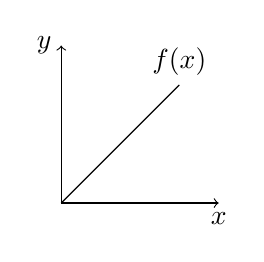
\begin{tikzpicture}
\draw[->] (0,0) -- (2,0) node [pos=1.0,below] {\(x\)};
\draw[->] (0,0) -- (0,2) node [pos=1.0,left] {\(y\)};
\draw (0,0) -- (1.5,1.5) node [pos=1.0,above] {\(f(x)\)};
\end{tikzpicture}
\caption{This is great caption}\label{figure}
\end{figure}\\
If you want to know more, check: \url{https://en.wikibooks.org/wiki/LaTeX/PGF/TikZ}.

%% If you want to include figure:
%\includegraphics[scale=1.0]{filename}
%% check https://en.wikibooks.org/wiki/LaTeX/Importing_Graphics if you want to know more

\end{document}
